\section{Présentation}
	Cet algorithme utilise à la fois des informations liées aux intensités des pixels et des informations spatiales. En effet, on cherche à minimiser deux énergies. Une première énergie est une fonction décroissante de la probabilité que l'intensité du pixel appartienne à la classe. On considère que cette probabilité suit une loi normale de moyenne égale à la moyenne des intensités des pixels de cette classe et de variance égale à la variance des intensités des pixels de cette classe. La deuxième énergie est liée au voisinage du pixel. Elle est égale à une certaine pénalité, choisie en paramètre, multipliée par le nombre de pixels présents dans le voisinage 3x3 n'étant pas de la classe.\\

	À chaque itération, on calcule la valeur des énergies pour chaque pixel, pour chaque classe, et on attribue à chaque pixel la classe minimisant cette énergie. On itère ainsi jusqu'à ce que le nombre de pixels changeant de classe soit très faible.\\

	Dans notre cas, on utilise 3 classes, représentant :

	\begin{itemize}
		\item la tumeur;
		\item le reste du cerveau;
		\item le fond.
	\end{itemize}
	\bigskip

	On initialise les classes de chaque pixel avec une méthode semi-manuelle: l'utilisateur choisit à la main une petite portion de la tumeur et une petite portion du cerveau. On calcule alors la moyenne et la variance des intensités de ces classes et on affecte les classes aux pixels en se basant uniquement sur l'énergie interne, utilisant la probabilité d'appartenance aux classes.\\

	En considérant que l'initialisation de l'utilisateur est fiable, le paramètre principal est la pénalité attribuée à chaque voisin de classe différente.

\section{Résultats}
	On applique cet algorithme avec une pénalité de 0.2. La figure \ref{fig:etapes} montre l'évolution de l'attribution des classes au fur et à mesure des itérations pour l'image correspondant à l'IRM avant traitement. 

	\begin{figure}[H]
		\centering
		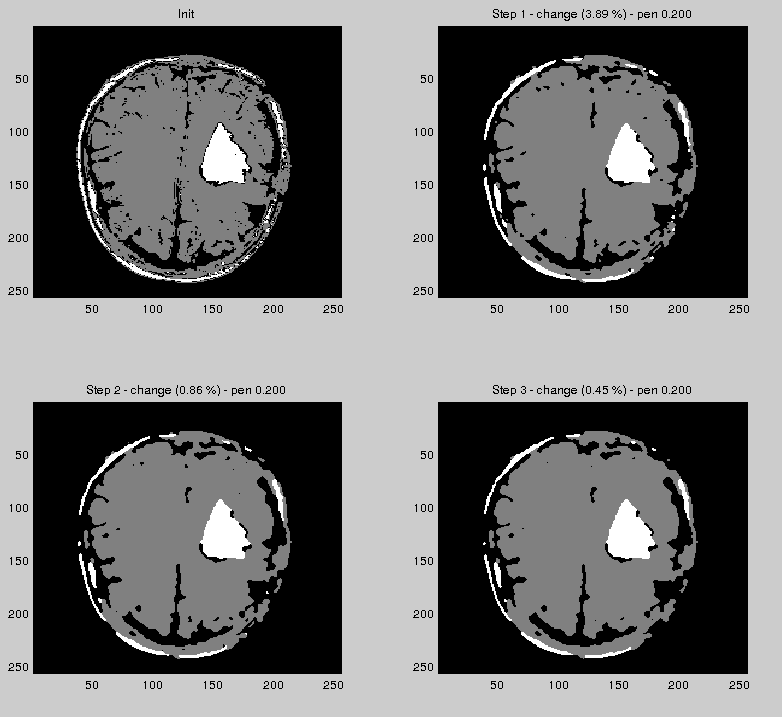
\includegraphics[width=0.7\textwidth]{images/3-etapes.png}.
		\caption{Étapes des champs de markov}
		\label{fig:etapes}
	\end{figure}

	On applique ensuite les mêmes techniques que précédemment afin d'identifier la tumeur. Les contours de la tumeur sont tracés dans la figure \ref{3irm1} pour l'IRM avant traitement et dans l'image \ref{3irm2} pour l'IRM après traitement.\\

	\begin{figure}[t!]
    \centering
    \begin{subfigure}[b]{0.5\textwidth}
        \centering
        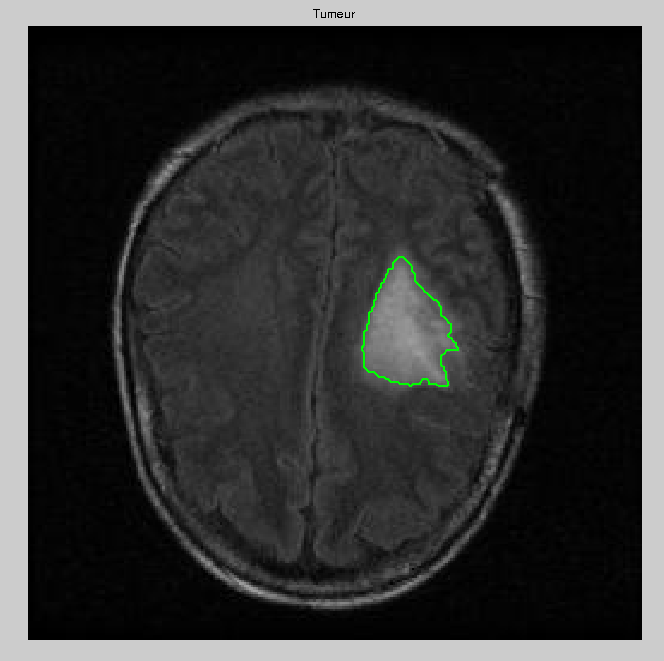
\includegraphics[width=0.95\textwidth]{images/3-tumeur1.png}
	\caption{Contours de la tumeur sur l'IRM avant traitement}\label{3irm1}
    \end{subfigure}%
    ~ 
    \begin{subfigure}[b]{0.5\textwidth}
        \centering
        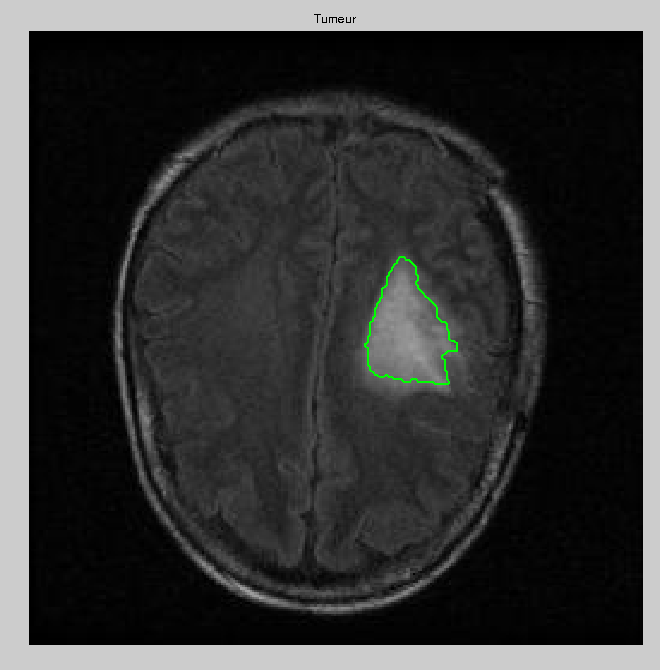
\includegraphics[width=0.95\textwidth]{images/3-tumeur2.png}
	\caption{Contours de la tumeur sur l'IRM après traitement}\label{3irm2}
    \end{subfigure}
\end{figure}

    On peut ainsi obtenir l'aire des tumeurs sur chacune des images, et on trouve que la surface de la tumeur a diminué de 6.76\%.

\section{Influence de la pénalité} % (fold)
\label{sub:influence_de_la_p_nalit_}
	Un paramètre important de cet algorithme est la pénalité attribuée à chaque voisin n'ayant pas la même classe que celle qu'on envisage d'attribuer au pixel. La figure \ref{fig:ratios} représente l'évolution du ratio d'augmentation de la taille de la tumeur lorsque la pénalité varie.

	\begin{figure}[H]
		\centering
		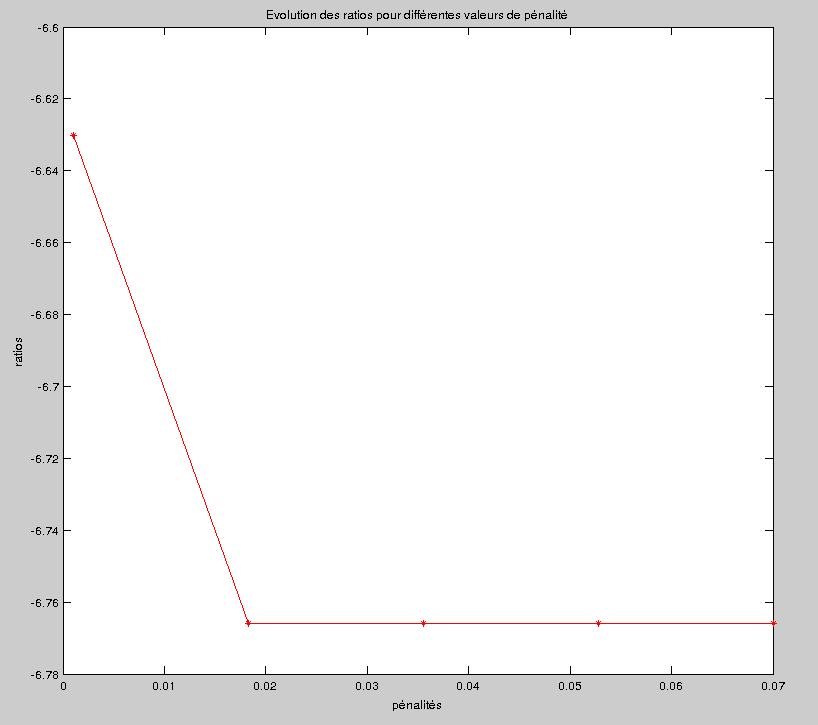
\includegraphics[width=0.8\textwidth]{images/3-ratios.png}.
		\caption{Comparaison du ratio pour différentes valeurs de pénalités}
		\label{fig:ratios}
	\end{figure}

	On constate qu'une fois que la pénalité est supérieure à 0.001, son évolution n'a plus d'effet ce qui signifie que l'algorithme est stable.

% section influence_de_la_p_nalit_ (end)